% Versión corta de defensa.tex para la predefensa: once láminas principales con los resultados
% más importantes y el resto como respaldo. Se genera con armar_corta.py a partir de defensa.tex.
\documentclass[aspectratio=169]{beamer}
\usepackage[utf8]{inputenc}
\usepackage[T1]{fontenc}
\usepackage[spanish,es-tabla]{babel}
\usepackage{booktabs,graphicx,tikz,amsmath,adjustbox,array}
\usetikzlibrary{arrows.meta,positioning}
\usepackage{tesis_beamer}

% Figuras: las del paper (especificación vigente) y, como respaldo, las de la tesis.
% En el zip para Prism todas viven en imagenes/. Las baterías se cargan desde tablas/
% (generadas por tablas_beamer.py a partir de las tablas de la tesis).
\graphicspath{{../envios/paper_empirico/figuras/}{../tesis/imagenes/}{imagenes/}}

% Una sola tabla de contenidos al inicio: sin la recapitulación automática por sección
\AtBeginSection[]{}

% Notación compartida con la tesis
\newcommand{\JLoss}{\mathrm{JLoss}}
\newcommand{\GaR}{\mathrm{GaR}}
\newcommand{\Spread}{\mathrm{spread}}
\newcommand{\EMBI}{\mathrm{EMBI}}
% Cifra destacada
\newcommand{\cifra}[2]{\begin{center}{\Huge\bfseries\color{tesisblue}#1}\\[2pt]{\small #2}\end{center}}
% Leyenda común de las baterías
\newcommand{\notabat}[1]{\par\vspace{3pt}{\scriptsize\raggedright
\textbf{Cómo leer:} variable dependiente $\ln\EMBI_{i,t}$. #1
Efectos fijos: P = país, T = tiempo (trimestre), PT = ambos. Ref.\ = especificación de referencia con EF país + tiempo.
Errores Driscoll--Kraay; *** $p<0{,}01$, ** $p<0{,}05$, * $p<0{,}10$. Celda vacía: la variable no está en ese modelo.\par}}

\author{Mauricio Valenzuela Corvalán}
\institute[Universidad de Chile]{Departamento de Ingeniería Civil Industrial\\
\small Magíster en Economía Aplicada · Universidad de Chile}
\title[Fragilidad bancaria y riesgo de cola]{Fragilidad bancaria sistémica y riesgo de cola del crecimiento}
\subtitle{Determinantes del \textit{spread} soberano en economías emergentes}
\date{Predefensa (versión corta) · \today}

\setbeamertemplate{navigation symbols}{}

\begin{document}
% =====================================================================
\begin{frame}
\titlepage
\vspace{-8pt}
\centering
\footnotesize Profesor guía: Juan Francisco Martínez Sepúlveda \quad\quad
Profesor coguía: Ronald Fischer
\end{frame}

\begin{frame}{Dos pilares del \textit{spread} soberano emergente}
\begin{exampleblock}{¿Qué es el \textit{spread} soberano?}
\footnotesize Diferencia entre el rendimiento de los bonos en dólares de un gobierno emergente y el del Tesoro de EE.UU.\ a igual plazo: la \textbf{prima que exige el mercado por el riesgo de incumplimiento} del país, en puntos básicos (EMBI Global Diversified, J.P.\ Morgan).
\end{exampleblock}
\vspace{-10pt}
\begin{columns}[T]
\column{0.48\textwidth}
\begin{block}{Fundamentos domésticos}
\footnotesize
\begin{itemize}
\item Edwards (1984); Hilscher y Nosbusch (2010); Uribe y Yue (2006).
\item \textbf{Proxies:} riesgo financiero ($\JLoss$) y riesgo económico ($\GaR$).
\end{itemize}
\end{block}
\column{0.48\textwidth}
\begin{block}{Factores globales}
\footnotesize
\begin{itemize}
\item Calvo et al.\ (1996); Longstaff et al.\ (2011); Miranda-Agrippino y Rey (2022).
\item \textbf{Proxy:} efectos fijos de tiempo (VIX, Tesoro, \textit{high yield}).
\end{itemize}
\end{block}
\end{columns}
\begin{alertblock}{La brecha}
\footnotesize Chari et al.\ (2024) ya documentan la fragilidad bancaria y la cruzan con factores globales. No se han cruzado \textbf{simultáneamente} los dos riesgos de cola domésticos: el financiero y el económico.
\end{alertblock}
\end{frame}

\begin{frame}{Pregunta e hipótesis}
\begin{block}{Pregunta}
Sobre la fragilidad bancaria que ya documentan Chari et al.\ (2024), ¿\textbf{qué agrega} el riesgo económico doméstico, y qué pasa cuando los dos riesgos \textbf{se dan a la vez}?
\end{block}
\vspace{4pt}
\begin{itemize}
\item \textbf{H1 (canal bancario).} La fragilidad bancaria sistémica eleva el \textit{spread} soberano.
\item \textbf{H2 (canal de crecimiento).} Un mayor riesgo de cola del crecimiento eleva el \textit{spread} soberano.
\item \textbf{H3 (amplificación).} La coincidencia de ambos riesgos eleva el \textit{spread} más que la suma de las dos asociaciones.
\end{itemize}
Además se contrasta si tres condiciones ---resiliencia, respaldo externo y quién tiene la deuda--- modifican la transmisión.
\vspace{4pt}
\footnotesize Matiz: aditivo en logaritmos es proporcional en puntos básicos. Esa complementariedad es álgebra de la forma funcional y \textbf{no} se llama amplificación; H3 exige una interacción positiva. Son asociaciones, no causalidad.
\end{frame}

\begin{frame}{Especificación principal y batería}
\begin{block}{Log-log rezagada}
\vspace{-6pt}
\[
\ln\EMBI_{i,t}=\alpha_i+\delta_t+\beta_1\ln\JLoss_{i,t-1}+\beta_2D_{i,t-1}+\beta_3\,(\ln\JLoss\times D)_{i,t-1}+\varepsilon_{i,t}
\]
\vspace{-8pt}
\end{block}
{\scriptsize \textbf{Donde:} $i$ país, $t$ trimestre; $\ln\EMBI$ logaritmo del \textit{spread} soberano; $\alpha_i$ efecto fijo de país; $\delta_t$ efecto fijo de tiempo; $D=-\GaR$ riesgo de cola (pp); $\beta_1$ elasticidad a la fragilidad; $\beta_2$ semielasticidad al riesgo de cola; $\beta_3$ interacción (amplificación adicional si $>0$); $\varepsilon$ error.\par}
\vspace{4pt}
\begin{columns}[T]
\column{0.5\textwidth}
\small
\textbf{Batería: 4 modelos anidados}
\begin{itemize}
\item M1: solo fragilidad \quad M2: solo cola
\item M3: ambas \quad M4: ambas + interacción
\end{itemize}
\column{0.48\textwidth}
\small
\textbf{× 3 efectos fijos × 3 muestras}
\begin{itemize}
\item EF: tiempo (T), país (P), ambos (PT)
\item Completa, sin crisis, con 6 controles
\end{itemize}
\end{columns}
\end{frame}

\begin{frame}{Lectura de la batería: réplica y validación del panel}
\begin{columns}[T]
\column{0.48\textwidth}
\cifra{0,10}{elasticidad a la fragilidad (columna 1)\\ una desviación estándar dentro del país $\approx$ +5\,\% (13 pb)}
\column{0.48\textwidth}
\cifra{0,107--0,164}{con los controles de Chari et al.\\ con el CDS en vez del EMBI: 0,206}
\end{columns}
\vspace{2pt}
\small
\begin{itemize}
\item \textbf{Se replica a Chari et al.\ con sus controles}, sobre datos construidos de forma independiente: es el punto de partida, no el hallazgo de la tesis.
\item Con los seis controles domésticos de la tesis (Panel C) la fragilidad se diluye: $-0{,}008$ ($p=0{,}86$).
\item Riesgo de cola: una desviación estándar dentro del país $\approx+10\%$ de \textit{spread}.
\item Ninguno de los tres coeficientes de la regresión principal resiste el \textit{wild bootstrap} ($p=0{,}33$ / $0{,}20$ / $0{,}89$); $\beta_3$ nunca es significativamente positivo.
\end{itemize}
\end{frame}

\begin{frame}{Qué agrega el riesgo económico a lo que explica la fragilidad}
\begin{columns}[T]
\column{0.56\textwidth}
\centering
\footnotesize
\begin{adjustbox}{max width=\textwidth}
\begin{tabular}{l ccc}
\toprule
$N=662$ & Fragilidad & + cola & + interacción \\
\midrule
Fragilidad ($\beta_1$) & $0{,}137^{***}$ & $0{,}107^{***}$ & $0{,}119^{***}$ \\
Riesgo de cola ($\beta_2$) & & $0{,}037^{***}$ & $0{,}041^{***}$ \\
\quad $p$ \textit{wild} & & $0{,}066$ & $0{,}11$ \\
Interacción ($\beta_3$) & & & $-0{,}015^{**}$ \\
\quad $p$ \textit{wild} & & & $0{,}58$ \\
$R^2$ dentro del país & $0{,}153$ & $0{,}185$ & $0{,}194$ \\
\bottomrule
\end{tabular}
\end{adjustbox}

\vspace{3pt}
{\scriptsize\raggedright Modelo de Chari et al.: fragilidad rezagada y sus controles; EF de país y de tiempo. Prueba conjunta $\beta_2=\beta_3=0$: $p$ \textit{wild} $=\mathbf{0{,}041}$. Sin controles ($N=765$): $0{,}030$ ($p$ \textit{wild} $0{,}17$). *** $p<0{,}01$, ** $p<0{,}05$ (Driscoll--Kraay).\par}
\column{0.42\textwidth}
\begin{alertblock}{Pero}
\footnotesize
\begin{itemize}\setlength\itemsep{0pt}
\item Cambios a cuatro trimestres: $0{,}004$ ($p$ \textit{wild} $0{,}13$).
\item Proyecciones locales: 0 de 9 horizontes. Entre países: $0{,}052$ ($p=0{,}46$).
\item Fuera de muestra: agregarlo sube el error un 3\% (evidencia débil: diseño sin efectos de tiempo).
\item El \textit{wild bootstrap} no protege del sesgo de retroalimentación: $+0{,}022$ simulado frente a $0{,}032$.
\end{itemize}
\end{alertblock}
\end{columns}
\vspace{1pt}
{\footnotesize\raggedright \textbf{Lectura (sugerente, solo en niveles):} una asociación modesta, de 0,02--0,03 por punto porcentual de riesgo de cola, que no mejora el pronóstico del \textit{spread} ni aparece en los cambios.\par}
\end{frame}

\begin{frame}{Los dos riesgos coinciden más de lo que explicaría el azar}
\centering
\footnotesize
\begin{adjustbox}{max width=\textwidth}
\begin{tabular}{l ccc}
\toprule
\textit{Ambos riesgos en su tercil alto (definido dentro de cada país)} & Observado & Por azar & $p$ \\
\midrule
Observaciones conjuntas ($22{,}0\%$ de 765) & \textbf{168} & 87 (independencia) & 1,9 veces \\
Permutación entre países dentro de cada trimestre (calendario común) & 168 & $140{,}9$ & \textbf{1,2 veces}; $0{,}0002$ \\
Permutación por bloques dentro de cada país (999 réplicas) & 168 & $85{,}7$ & $0{,}001$ \\
Fuera de los trimestres de crisis & 108 & $59{,}3$ & $0{,}001$ \\
Duración media de los 62 episodios conjuntos (trimestres) & $2{,}71$ & $1{,}85$ & $0{,}003$ \\
Países con más coincidencias que las esperadas & \textbf{13 de 13} & & \\
\midrule
\textit{Rezago cruzado (rezago propio, EF de país y de tiempo)} & Coeficiente & & $p$ \textit{wild} \\
\midrule
Fragilidad en $t-1$ $\to$ riesgo de cola en $t$ & $\mathbf{0{,}405^{***}}$ & & $0{,}024$ \\
\quad sin cada país (rango) / con el $GaR$ sin bloque bursátil & $[0{,}32;\,0{,}47]$ / $0{,}388$ & & DK $<0{,}07$ / $0{,}002$ \\
Riesgo de cola en $t-1$ $\to$ fragilidad en $t$ & $-0{,}006$ & & $0{,}48$ \\
\bottomrule
\end{tabular}
\end{adjustbox}
\vspace{-2pt}
\begin{columns}[T]
\column{0.56\textwidth}
\begin{block}{Lectura}
\footnotesize \textbf{Simultaneidad: firme}, 1,2 veces lo esperado (calendario común). \textbf{Precedencia: firme a un trimestre}, sin depender de un país ni del bloque bursátil; pequeña y no causal.
\end{block}
\column{0.42\textwidth}
\begin{alertblock}{Salvedad}
\footnotesize Pocos episodios comunes: 129 de las 168 son de 2020 en adelante; el exceso sobre lo esperado viene de 2015--19 y 2023--26.
\end{alertblock}
\end{columns}
\end{frame}

\begin{frame}{Cuando coinciden, no hay evidencia de que se amplifiquen}
\centering
\footnotesize
\begin{adjustbox}{max width=\textwidth}
\begin{tabular}{l cc}
\toprule
Prueba & Estimación & $p$ \textit{wild bootstrap} \\
\midrule
Interacción $\beta_3$ de la regresión principal & $-0{,}011$ & $0{,}89$ \\
Estrés conjunto: extra con los dos riesgos altos (fragilidad alta $+0{,}091$; cola alta $+0{,}186$) & $-0{,}077$ & $0{,}23$ \\
Estrés conjunto uno a cuatro trimestres adelante & $-0{,}097$ a $-0{,}046$ & $0{,}17$ a $0{,}37$ \\
Estrés conjunto con cuartiles en vez de terciles & $-0{,}122$ & $0{,}23$ \\
Forma funcional intermedia (Box--Cox, $\lambda=0{,}44$): interacción & $t=-0{,}19$ & $0{,}97$ \\
\bottomrule
\end{tabular}
\end{adjustbox}
\vspace{3pt}
\begin{itemize}\footnotesize\setlength\itemsep{2pt}
\item Es un no rechazo: una prueba de equivalencia descarta una amplificación de más de un 35\% de la suma, no una menor (lámina siguiente).
\item El signo negativo de $\beta_3$ es de \textbf{Polonia} (sin ella $+0{,}008$, $p=0{,}19$): \textbf{no} se lee como atenuación.
\item Aditivo en logaritmos es proporcional en puntos básicos: es álgebra de la forma funcional, no un hallazgo.
\item \textbf{Señales débiles en contra}, que se reportan: fuera del piso de $\JLoss$ el riesgo de cola pesa $+7{,}5$ pb más ($p$ \textit{wild} $0{,}036$) con un umbral de 2\%, y en logaritmos no ($0{,}11$); en cambios a cuatro trimestres en pb la interacción es $+0{,}358$ ($0{,}011$), ausente en logaritmos.
\end{itemize}
\end{frame}

\begin{frame}{Deuda y riesgo de cola: lo que resiste y lo que no}
\centering
\scriptsize
\begin{adjustbox}{max width=\textwidth, max totalheight=0.60\textheight}
\begin{tabular}{>{\raggedright\arraybackslash}p{0.34\textwidth}>{\raggedright\arraybackslash}p{0.40\textwidth}>{\raggedright\arraybackslash}p{0.18\textwidth}}
\toprule
Prueba & Resultado & Lectura \\
\midrule
Preregistro 1: riesgo de cola a un trimestre $\times$ deuda & $+0{,}011$ por d.e. de deuda (de $0{,}043$ a $0{,}054$); Holm $0{,}029$; 13 de 13 & firme en su familia \\
Preregistro 2: riesgo de cola a un año & $0{,}047$ (Holm $0{,}018$); $\times$ deuda $+0{,}033$: una d.e.\ más de deuda, $+70\%$ & firme en su familia \\
\addlinespace
Inferencia conjunta (14 hipótesis, 4 preregistros) & ninguna bajo $0{,}05$; permutación de la deuda: a un trimestre $0{,}17$, a un año $0{,}009$ & a un año resiste \\
Corrección sobre los 8 preregistros (23 hipótesis) & riesgo de cola a un año: Holm $0{,}13$; deuda $\times$ cola: $0{,}31$ & no sobreviven \\
\addlinespace
Réplica externa: Hungría y Corea & $0{,}22$ frente a $0{,}033$; diferencia rechazada; potencia 5\% & \textbf{no replica} \\
Instrumento: términos de intercambio & F $20$ para el riesgo de cola, $9{,}7$ para la interacción; $\psi\approx0$ & \textbf{débil} \\
Modelo de límite fiscal calibrado & logaritmos: $-0{,}43$; puntos básicos: $+91$ (dato $+3{,}1$) & \textbf{no lo explica} \\
\bottomrule
\end{tabular}
\end{adjustbox}
\vspace{2pt}
\begin{block}{Lectura}
\scriptsize Con más deuda, el riesgo de cola del año siguiente pesa más en el \textit{spread} \textbf{en la muestra}. Fuera de ella, con un instrumento o con un modelo, nada lo confirma por ahora. Se reporta como lo que es: una regularidad de la muestra.
\end{block}
\end{frame}

\begin{frame}{Hallazgos y su grado de evidencia}
\centering
\renewcommand{\arraystretch}{1.4}
\begin{adjustbox}{width=\textwidth, max totalheight=0.84\textheight}
\begin{tabular}{lll}
\toprule
\textbf{Hallazgo} & \textbf{Cifra} & \textbf{Evidencia} \\
\midrule
Los dos riesgos coinciden & 1,2 veces lo esperado ($p=0{,}0002$) & \textbf{Firme} \\
La fragilidad antecede a la cola & $0{,}405$ (\textit{wild} $0{,}024$) & \textbf{Firme} (1 trim.) \\
Amplificación (H3) & $-0{,}011$; se descarta $>35\%$ & \textbf{No hay evidencia} \\
El riesgo de cola agrega (H2) & $0{,}032$; CCE \textit{wild} $0{,}016$ & Firme como nivel \\
Fragilidad y \textit{spread} (H1) & $0{,}099$; 70\% es Turquía & Sugerente \\
Deuda $\times$ cola, en la muestra & $+0{,}033$ (permutación $0{,}009$) & Firme en la muestra \\
Deuda $\times$ cola, fuera de ella & réplica, instrumento y modelo & \textbf{No se confirma} \\
Otros moderadores y umbrales & Holm $\geq0{,}29$ & \textbf{No hay evidencia} \\
Corrección global (23 hipótesis) & riesgo de cola a un año $0{,}13$; deuda $\times$ cola $0{,}31$ & \textbf{No sobreviven} \\
\bottomrule
\end{tabular}
\end{adjustbox}
\end{frame}

\begin{frame}{Implicancias}
\begin{columns}[T]
\column{0.48\textwidth}
\begin{block}{Respaldado por los datos}
\small
\textbf{Vigilar los dos riesgos juntos} se justifica: tienden a agravarse a la vez, y la fragilidad bancaria antecede al deterioro de la cola del crecimiento.
\end{block}
\column{0.48\textwidth}
\begin{exampleblock}{Sin base en estos datos}
\small
\begin{itemize}
\item Una prima adicional por la simultaneidad.
\item Recomendar la acumulación de reservas.
\item Diferenciar por quién tiene la deuda.
\item Un umbral de vigilancia o un semáforo.
\end{itemize}
\end{exampleblock}
\end{columns}
\vspace{8pt}
\begin{alertblock}{No permite}
Cuantificar cuánto bajaría el \textit{spread} si cae la fragilidad: son asociaciones, y el \textit{spread} también retroalimenta a los bancos.
\end{alertblock}
\end{frame}

\begin{frame}{Conclusión}
\vspace{4pt}
\begin{enumerate}
\item Los dos riesgos domésticos \textbf{coinciden}, también descontado el calendario común, y la fragilidad bancaria antecede al riesgo económico.
\vspace{4pt}
\item Cuando coinciden, \textbf{no hay evidencia de amplificación}, se descarta más de un 35\% de la suma, aunque no menos.
\vspace{4pt}
\item El riesgo económico \textbf{agrega poco} a lo que ya explica la fragilidad, pero es un fundamento de largo plazo.
\vspace{4pt}
\item Con más \textbf{deuda}, el riesgo de cola pesa más \textbf{en la muestra}; ni la réplica externa, ni el instrumento, ni el modelo lo confirman.
\end{enumerate}
\vspace{4pt}
{\small \textbf{Réplica:} la asociación fragilidad--\textit{spread} replica a Chari et al.\ con sus controles, pero no es una elasticidad común ni hay precedencia temporal.\par}
\vspace{6pt}
\centering
\textit{El aporte es el primer cruce de los dos riesgos domésticos, evaluado con ocho preregistros: qué se puede afirmar, y qué no, con 13 países.}
\end{frame}

\begin{frame}
\vfill
\centering
{\Huge\bfseries\color{tesisblue} Gracias}
\vfill
\end{frame}

% =====================================================================
\appendix

\begin{frame}{Respaldo: Qué aporta esta tesis}
\small
\begin{block}{Las métricas no son mías; la construcción de las series y su cruce, sí}
\footnotesize $\JLoss$ es la métrica de \textbf{Chari et al.\ (2024)}; el $\GaR$, la de \textbf{Adrian, Boyarchenko y Giannone (2019)}, con la plataforma de CEMLA (Ossandón Busch et al., 2022). Que la fragilidad bancaria importa para el \textit{spread} ya lo establecen Chari et al.: aquí es el punto de partida.
\end{block}
\begin{enumerate}\setlength\itemsep{2pt}
\item \textbf{Series:} construcción homogénea y reproducible de las dos métricas para 13 economías (113 bancos, un solo protocolo de Bloomberg; $\GaR$ en pseudo--tiempo real).
\item \textbf{Réplica independiente} de Chari et al.\ y delimitación de su alcance: no es una elasticidad común y no hay precedencia temporal.
\item \textbf{Primer cruce} de la fragilidad bancaria con el riesgo de cola doméstico: coinciden, la fragilidad antecede al riesgo de cola, no hay evidencia de que se amplifiquen y el riesgo económico agrega poco.
\item \textbf{Ocho preregistros} fechados antes de los datos: cada resultado se reporta salga como salga.
\item \textbf{Teoría frente a datos:} un modelo de límite fiscal muestra que la predicción sobre deuda y riesgo de cola es en pb, no en logaritmos.
\end{enumerate}
\end{frame}

\begin{frame}{Respaldo: Construcción de $\JLoss$: fragilidad bancaria sistémica}
\small
Pérdida conjunta esperada del sistema bancario ante un evento sistémico, en \% de la exposición (Chari et al., 2024).
\begin{enumerate}
\item \textbf{Probabilidad de incumplimiento de cada banco} (Merton--KMV): $D^*=L_{ST}+\tfrac12L_{LT}$,\quad $EDF=\Phi(-DD)$.
\item \textbf{Factor sistémico} país (Vasicek): $p_i(V)=\Phi\!\left(\frac{\Phi^{-1}(p_i)-\rho_iV}{\sqrt{1-\rho_i^2}}\right)$.
\item \textbf{Agregación por punto de silla} de la distribución de pérdidas del sistema.
\item \textbf{Métrica}: $\JLoss=\dfrac{EL+UL}{\sum_j EAD_j}\times100$.
\end{enumerate}
\vspace{2pt}
{\scriptsize \textbf{Donde:} $D^*$ punto de incumplimiento; $L_{ST}$, $L_{LT}$ pasivos de corto y largo plazo; $DD$ distancia al incumplimiento; $EDF$ frecuencia esperada de incumplimiento; $\Phi$ distribución normal estándar; $p_i$ PD del banco $i$; $V$ factor sistémico (retorno bursátil del país); $\rho_i$ correlación del banco con $V$; $EL$ pérdida esperada; $UL$ pérdida inesperada al 99\%; $EAD$ exposición; LGD $=45\%$. La cota de la malla es activa en el 98\% de los casos $\Rightarrow$ $\JLoss$ es \textbf{ordinal} y entra en logaritmos.\par}
\end{frame}

\begin{frame}{Respaldo: Construcción del $\GaR$: riesgo de cola del crecimiento}
\begin{columns}[c]
\column{0.52\textwidth}
\footnotesize
\begin{enumerate}
\item \textbf{Índice de condiciones financieras} (FCI tipo CISS): tensión accionaria, de tasas y cambiaria, en términos reales (deflactadas por la inflación).
\item \textbf{Regresión cuantílica de panel}, un trimestre adelante:\\
{\footnotesize $Q(\Delta y_{i,t+1}\mid\cdot;\tau)=\alpha+\beta_1\Delta y_{i,t}+\beta_2FCI^{\perp}_{i,t}+\beta_3VIX_t+\mu_i$}
\item $\GaR_{i,t}$ = cuantil $\tau=5\%$; ventana expansiva (pseudo--tiempo real).
\end{enumerate}
\vspace{2pt}
{\scriptsize \textbf{Donde:} $Q(\cdot;\tau)$ cuantil $\tau$ del crecimiento; $\Delta y$ crecimiento del PIB; $FCI^{\perp}$ FCI sin el componente del VIX; $\mu_i$ efecto fijo de país. En la tesis $D\equiv-\GaR$: mayor $D$, cola más adversa. No es circular con el EMBI (corr.\ 0,985 sin el componente tipo \textit{spread}).\par}
\column{0.46\textwidth}
\centering
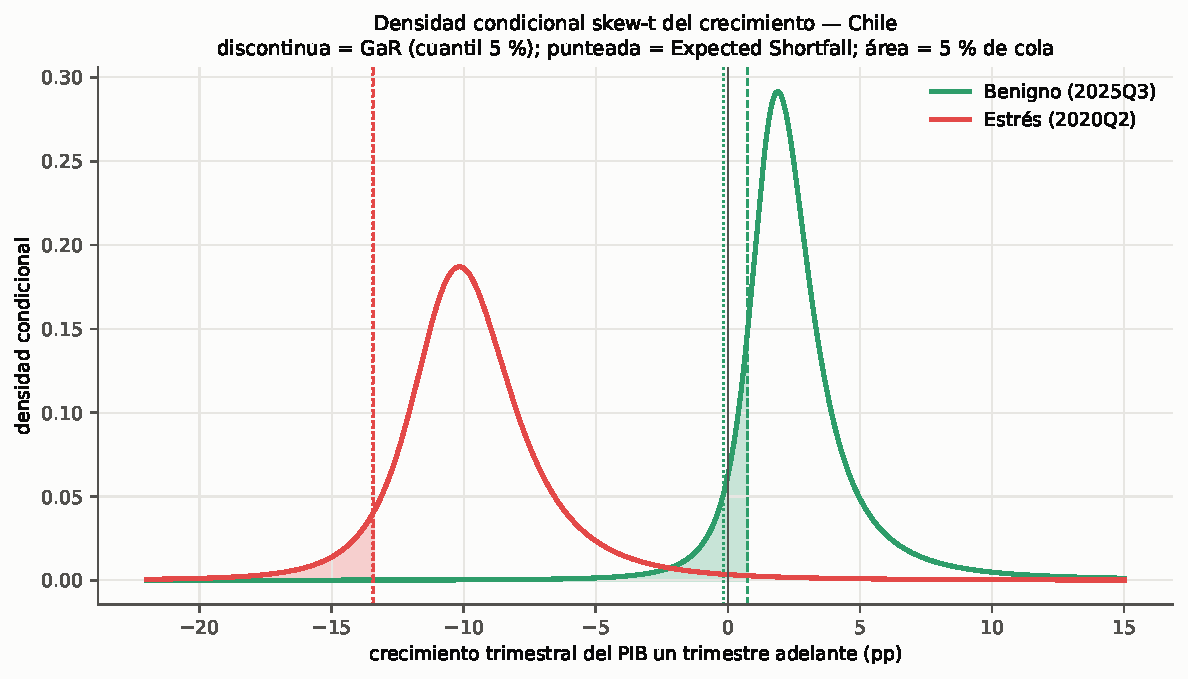
\includegraphics[width=\textwidth]{fig_skewt_chile_embiext.pdf}\\
{\scriptsize Chile: trimestre benigno vs.\ 2020Q2 ($\GaR=-13{,}4$ pp).}
\end{columns}
\end{frame}

\begin{frame}{Respaldo: Inferencia: cómo mido la incertidumbre}
\footnotesize
\begin{itemize}\setlength\itemsep{1pt}
\item \textbf{Driscoll--Kraay (referencia de las tablas):} robustos a heterocedasticidad, autocorrelación y choques comunes entre países.
\item \textbf{\textit{Cluster} por país} y \textbf{\textit{wild cluster bootstrap}} por país (pesos de Webb, 1\,999 réplicas): los contrastes exigentes con 13 países.
\item \textbf{Calibración por simulación:} 1\,000 paneles simulados miden cuánto rechaza de más cada método. En niveles, el criterio es el \textit{wild bootstrap}.
\item \textbf{Permutación por bloques} para la simultaneidad; \textbf{corrección de Holm} para las familias de contrastes.
\item \textbf{Prueba preespecificada:} la de la participación extranjera se fijó antes de estimar.
\item \textbf{Identificación:} canal inverso, fechas del \textit{spread} (promedio o cierre), cambios, proyecciones locales y pronóstico fuera de muestra.
\end{itemize}
\vspace{-7pt}
\begin{exampleblock}{Una sola escala de evidencia}
\footnotesize \textbf{Firme}: resiste el \textit{wild bootstrap} o la permutación y no depende de un país. \textbf{Sugerente}: solo Driscoll--Kraay, o depende de un país. \textbf{Exploratorio}: no preespecificado y no pasa la corrección de Holm. \textbf{No hay evidencia.}
\end{exampleblock}
\end{frame}

\begin{frame}{Respaldo: Las bandas: cuánta amplificación se descarta y cuánta no}
\begin{columns}[c]
\column{0.3\textwidth}
\cifra{+16,4\,\%}{de \textit{spread}: suma de las dos asociaciones (28 pb)}
\column{0.68\textwidth}
\centering
\small
\begin{adjustbox}{max width=\textwidth}
\begin{tabular}{l cccc}
\toprule
Intervalo de 95\% & $\beta_3$ & Extra máximo & \% de la suma & TOST: se rechaza más de \\
\midrule
Driscoll--Kraay & $[-0{,}025;\,0{,}003]$ & $+0{,}5$ puntos & 3\% & 0,4\% \\
\textit{Wild bootstrap} & $[-0{,}054;\,0{,}015]$ & $+2{,}9$ puntos & 16\% & 13\% \\
\textit{Cluster} por país & $[-0{,}050;\,0{,}028]$ & $+5{,}3$ puntos & 29\% & 22\% \\
En pb (\textit{wild}) & & $+11$ pb & 39\% & 35\% \\
\bottomrule
\end{tabular}
\end{adjustbox}
\end{columns}
\vspace{2pt}
{\footnotesize\raggedright Con ambos riesgos una desviación estándar dentro del país sobre su media. Extra estimado por la interacción: $-2{,}1$ puntos en logaritmos; en puntos básicos, $+3{,}0$ sobre 28. ``Extra máximo'': la mayor amplificación que el intervalo no permite descartar. TOST: la menor amplificación que se rechaza al 5\% (intervalo al 90\%).\par}
\vspace{-2pt}
\begin{alertblock}{Lo que se puede decir}
\footnotesize \textbf{No hay evidencia de amplificación}; se descarta una amplificación de más de un 35\% de la suma con los tres métodos y en las dos formas, pero no una menor.
\end{alertblock}
\end{frame}

\begin{frame}{Respaldo: Un modelo de límite fiscal: logaritmos frente a puntos básicos}
\small
\begin{columns}[T]
\column{0.52\textwidth}
\textbf{Modelo} (Eaton--Gersovitz; Bi, 2012)
\[ \text{incumple si } g<g^*(b)=\frac{r\,b-\bar p}{b+\bar p} \]
\[ \pi=\Phi\!\left(\frac{g^*-m}{\sigma_L}\right) \]
Más riesgo de cola: más $\sigma_L$, con la mediana fija.
\begin{itemize}\footnotesize
\item \textbf{Puntos básicos:} con más deuda, $g^*$ se acerca a la zona que la cola desplaza $\Rightarrow$ interacción \textbf{positiva}.
\item \textbf{Logaritmos:} con poca deuda el incumplimiento es de la cola profunda y ensancharla lo multiplica $\Rightarrow$ interacción \textbf{negativa}.
\end{itemize}
\column{0.44\textwidth}
\footnotesize
\textbf{Calibrado con el panel} (deuda 44,6\%, spread 173 pb, recuperación 63\%)
\vspace{2pt}

\begin{tabular}{lcc}
\toprule
 & Modelo & Datos \\
\midrule
Interacción, log & $-0{,}43$ & $+0{,}033$ \\
Interacción, pb & $+91$ & $+3{,}1$ \\
Riesgo de cola, log & $0{,}82$ & $0{,}047$ \\
\bottomrule
\end{tabular}
\vspace{4pt}

El modelo predice el signo contrario en logaritmos y una magnitud mucho mayor en pb. La forma funcional no es neutral.
\end{columns}
\end{frame}

\begin{frame}{Respaldo: Preguntas de portafolio y corrección global (preregistros 7 y 8)}
\centering
\footnotesize
\begin{adjustbox}{max width=\textwidth, max totalheight=0.54\textheight}
\begin{tabular}{>{\raggedright\arraybackslash}p{0.24\textwidth}>{\raggedright\arraybackslash}p{0.47\textwidth}>{\raggedright\arraybackslash}p{0.23\textwidth}}
\toprule
Prueba (mensual, desde 2015) & Resultado & Qué cambia \\
\midrule
Señal de valor relativo (Q1) & La fragilidad no ordena los retornos entre países: Sharpe bruto $+0{,}01$, neto $-4{,}07$ & La precedencia mensual no es una señal entre países \\
\addlinespace
Cola de los cambios del \textit{spread} (Q3) & Fragilidad alta la ensancha ($+0{,}062$; $p=0{,}005$), cola alta apenas ($+0{,}019$; $0{,}085$); la coincidencia no: $-0{,}046$ ($0{,}97$). El VaR condicional no mejora al EWMA ($p=0{,}47$) & Simultaneidad sin amplificación, también en la cola de los cambios \\
\addlinespace
Valor razonable (Q2) y cobertura condicional (Q4) & Clark--West $p=0{,}24$; frente a un beta móvil, $p=0{,}13$ & Los fundamentos describen niveles, no pronostican cambios \\
\addlinespace
\textit{Nowcast} del $\GaR$ (Q6) y deuda en pb (Q5) & Correlación $0{,}42$ con el $\GaR$ oficial (criterio $>0{,}9$): no valida; interacción en pb $-1{,}1$ ($p=0{,}73$) & Nada \\
\bottomrule
\end{tabular}
\end{adjustbox}
\vspace{2pt}
\begin{block}{Corrección sobre las 23 hipótesis primarias de los ocho preregistros}
\scriptsize Con Holm queda una sola bajo el 5\%: el signo de la réplica en Hungría y Corea ($0{,}046$), que no cambia su veredicto porque la magnitud es siete veces la original. Le siguen el riesgo de cola a un año ($0{,}13$) y la deuda $\times$ riesgo de cola ($0{,}31$). Con Benjamini--Yekutieli, ninguna.
\end{block}
\end{frame}

\begin{frame}{Respaldo: ¿Efecto o persistencia? La retroalimentación}
\begin{columns}[c]
\column{0.55\textwidth}
\centering
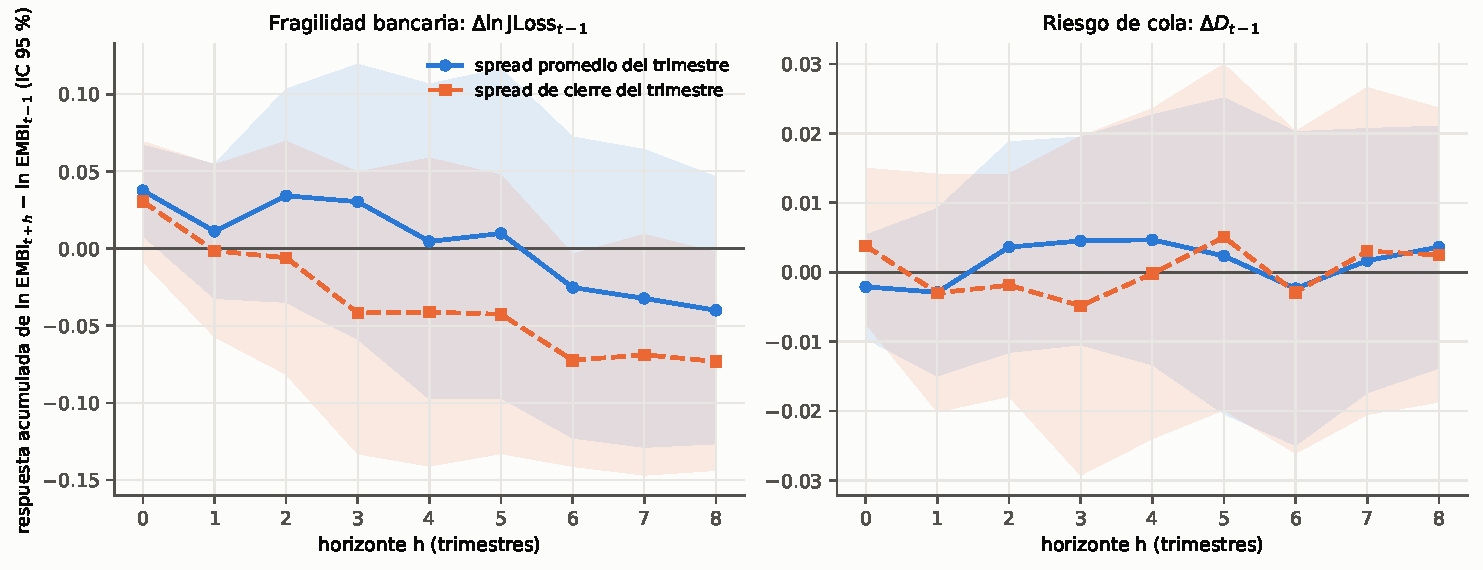
\includegraphics[width=\textwidth]{fig_lp_acumulada_lnlag.pdf}\\
{\scriptsize Proyecciones locales acumuladas: respuesta del \textit{spread} al cambio de la fragilidad (izq.) y del riesgo de cola (der.).}
\column{0.43\textwidth}
\footnotesize
\begin{itemize}\setlength\itemsep{2pt}
\item El \textit{spread} de ayer predice la fragilidad de hoy: \textbf{0,17} ($p=0{,}009$).
\item \textbf{Sesgo de retroalimentación}: en un panel simulado donde la fragilidad no tiene efecto directo, la regresión en niveles entrega $+0{,}066$ en promedio (dato: $0{,}099$). Para el riesgo de cola: $+0{,}022$ (dato: $0{,}032$).
\item \textbf{Nivel o cambio}: los datos no informan. Multiplicador de largo plazo $-0{,}146$, IC 95\% $[-0{,}79;\,0{,}50]$.
\item Proyecciones locales: solo el impacto con el \textit{spread} promedio ($0{,}038$); con el de cierre, nunca positiva y significativa. Riesgo de cola: plano.
\end{itemize}
\end{columns}
\end{frame}

\begin{frame}{Respaldo: Limitaciones y trabajo futuro}
\begin{columns}[T]
\column{0.48\textwidth}
\begin{alertblock}{Limitaciones}
\small
\begin{itemize}
\item 13 países: en niveles solo el \textit{wild bootstrap} está bien calibrado, con potencia de 35\% y 67\%.
\item Cada coeficiente de nivel depende de un país y tiene sesgo de retroalimentación.
\item El piso de $\JLoss$: un cuarto de las observaciones no informa (con la DD de Merton la asociación mejora; la interacción sigue nula).
\item La simultaneidad se concentra desde 2020.
\item Datos trimestrales: no separan la precedencia dentro del trimestre.
\end{itemize}
\end{alertblock}
\column{0.48\textwidth}
\begin{block}{Trabajo futuro}
\small
\begin{itemize}
\item Más economías (con EMBI directo, no imputado).
\item Frecuencia diaria y un $\GaR$ mensual.
\item La distancia al incumplimiento como medida principal, con la batería completa.
\item Variación exógena bancaria (el instrumento granular fue débil).
\item Más eventos de respaldo.
\end{itemize}
\end{block}
\end{columns}
\end{frame}

\begin{frame}{Respaldo: Panel A con errores estándar}
\centering
\begin{adjustbox}{max totalheight=0.72\textheight}
% Generado por tablas_beamer.py a partir de las tablas de la tesis; no editar a mano.
\begingroup\setlength{\tabcolsep}{3pt}\renewcommand{\arraystretch}{1.3}%
\begin{adjustbox}{max width=0.97\textwidth}
\begin{tabular}{l c ccc ccc ccc cc}
\toprule
 & Ref. & \multicolumn{3}{c}{M1} & \multicolumn{3}{c}{M2} & \multicolumn{3}{c}{M3} & \multicolumn{2}{c}{M4} \\
\cmidrule(lr){2-2}\cmidrule(lr){3-5}\cmidrule(lr){6-8}\cmidrule(lr){9-11}\cmidrule(lr){12-13}
Efectos fijos & PT & T & P & PT & T & P & PT & T & P & PT & T & P \\
 & (1) & (2) & (3) & (4) & (5) & (6) & (7) & (8) & (9) & (10) & (11) & (12) \\
\midrule
Fragilidad, $\beta_1$ & $0{,}0985^{***}$ & $0{,}1975^{***}$ & $0{,}1964^{***}$ & $0{,}1270^{***}$ &  &  &  & $0{,}2418^{***}$ & $0{,}1524^{***}$ & $0{,}0970^{***}$ & $0{,}2449^{***}$ & $0{,}1519^{***}$ \\
 & $(0{,}0330)$ & $(0{,}0318)$ & $(0{,}0420)$ & $(0{,}0378)$ &  &  &  & $(0{,}0366)$ & $(0{,}0414)$ & $(0{,}0317)$ & $(0{,}0345)$ & $(0{,}0433)$ \\
Riesgo de cola, $\beta_2$ & $0{,}0324^{**}$ &  &  &  & $0{,}0441^{***}$ & $0{,}0277^{***}$ & $0{,}0366^{**}$ & $0{,}0527^{***}$ & $0{,}0151^{*}$ & $0{,}0301^{*}$ & $0{,}0552^{***}$ & $0{,}0174^{*}$ \\
 & $(0{,}0152)$ &  &  &  & $(0{,}0151)$ & $(0{,}0093)$ & $(0{,}0170)$ & $(0{,}0164)$ & $(0{,}0087)$ & $(0{,}0165)$ & $(0{,}0160)$ & $(0{,}0097)$ \\
\textbf{Interacción}, $\beta_3$ & $-0{,}0112$ &  &  &  &  &  &  &  &  &  & $-0{,}0163$ & $-0{,}0059$ \\
 & $(0{,}0070)$ &  &  &  &  &  &  &  &  &  & $(0{,}0129)$ & $(0{,}0079)$ \\
\addlinespace
Observaciones & 765 & 765 & 765 & 765 & 765 & 765 & 765 & 765 & 765 & 765 & 765 & 765 \\
\bottomrule
\end{tabular}
\end{adjustbox}\endgroup

\end{adjustbox}
\notabat{Errores estándar Driscoll--Kraay entre paréntesis.}
\end{frame}

\begin{frame}{Respaldo: Hallazgos y su grado de evidencia}
\centering
\footnotesize
\begin{adjustbox}{max width=\textwidth, max totalheight=0.84\textheight}
\begin{tabular}{llc}
\toprule
Hallazgo & Cifra & Evidencia \\
\midrule
\multicolumn{3}{l}{\textit{Conclusiones propias}} \\
Los dos riesgos coinciden más que por azar & 168: 1,2 veces lo esperado con el calendario común ($p=0{,}0002$); 1,9 bajo independencia; 13 de 13 & \textbf{firme} \\
La fragilidad antecede al riesgo de cola & $0{,}405$ (\textit{wild} $0{,}024$); sin cada país y sin bloque bursátil & firme (a un trimestre) \\
Amplificación cuando coinciden & $-0{,}011$ (\textit{wild} $0{,}89$); TOST: se descarta $>35\%$ & \textbf{no hay evidencia} \\
El riesgo de cola agrega a la fragilidad, en niveles & conjunta \textit{wild} $0{,}041$; con cargas heterogéneas (CCE) \textit{wild} $0{,}016$, 13 de 13; largo plazo $0{,}067$ & firme como nivel; no en cambios \\
Deuda $\times$ riesgo de cola (preregistrada) & $+0{,}011$, de $0{,}043$ a $0{,}054$ (Holm $0{,}029$; conjunta $0{,}19$; 23 hipótesis $0{,}31$; permutación $0{,}17$); a 4 trimestres $+0{,}033$ (permutación $0{,}009$) & \textbf{firme} a 4 trim.\ en la muestra; sugerente a 1 \\
Réplica externa (Hungría, Corea) / instrumento de términos de intercambio & $0{,}22$, difiere de $0{,}033$ (potencia 5\%) / F $9{,}7$, interacción $\approx0$ & \textbf{no confirma} \\
Modelo de límite fiscal (preregistro 6) & log: predice $-0{,}43$ (dato $+0{,}033$); pb: predice $+91$ (dato $+3{,}1$, \textit{wild} $0{,}09$) & \textbf{no lo explica} \\
Riesgo de cola a 4 trimestres (preregistrada) & $0{,}047$; Holm $0{,}018$; 13 de 13; con las 23 hipótesis, Holm $0{,}13$ & \textbf{firme} en su familia \\
\textit{Doom loop} (deuda $\times$ fragilidad) / pecado original & $-0{,}053$ / $-0{,}004$; Holm $1{,}00$ & no hay evidencia \\
El riesgo de cola en cambios o fuera de muestra & $0{,}004$; 0 de 9 horizontes; $+3\%$ de error & \textbf{no hay evidencia} \\
Resiliencia: directa y con la cola fuera de crisis & $-0{,}153$; $-0{,}024$; solo Driscoll--Kraay & sugerente \\
Reservas $\times$ fragilidad & $-0{,}247$ (\textit{wild} $0{,}08$); preregistrada con adecuación de reservas: Holm $0{,}29$ & exploratorio \\
Resiliencia previa $\times$ riesgo de cola & $-0{,}028$ (\textit{wild} $0{,}06$) & exploratorio \\
Amplificación en el núcleo de 11, sin crisis & $+0{,}034$ (\textit{wild} $0{,}015$); grupo \textit{ex post} & exploratorio \\
Participación extranjera (preespecificada) & Holm $p=1{,}00$ & \textbf{no hay evidencia} \\
Respaldo externo por país & $-0{,}004$ (\textit{wild} $0{,}90$) & \textbf{no hay evidencia} \\
Eventos diarios de respaldo & \textit{swap} Fed 2020: $-20$ a $-22$ pp; desacople igual que sin línea & baja el nivel; \textbf{no} la transmisión \\
Asimetría \textit{Backstop} / \textit{EMstress} & Holm $0{,}12$ / $0{,}24$; lugar 20 de 51 & \textbf{no hay evidencia} \\
Umbrales de vigilancia (preregistrada) & tensión $p=0{,}13$; deuda $0{,}26$; AUROC fuera de muestra $0{,}49$; por país, no comunes & \textbf{no hay evidencia} \\
Cola de los cambios del \textit{spread} (preregistrada) & cada riesgo la ensancha; la coincidencia no: $-0{,}046$ ($p=0{,}97$) & \textbf{no hay evidencia} \\
Señales de mercado (preregistradas) & valor relativo: Sharpe neto $-4{,}07$; valor razonable: Clark--West $p=0{,}24$; cobertura: $p=0{,}13$ & \textbf{no hay evidencia} \\
\midrule
\multicolumn{3}{l}{\textit{Réplica de Chari et al.\ (2024) y validación del panel}} \\
Fragilidad y \textit{spread} en niveles & $0{,}099$ (\textit{wild} $0{,}33$); $0{,}107$--$0{,}164$ con sus controles; 70\% es Turquía; con la DD de Merton, \textit{wild} $0{,}055$ & sugerente \\
La fragilidad antecede al \textit{spread} & trimestral: cierre a cierre $0{,}025$ (\textit{wild} $0{,}21$); mensual: $0{,}013$ a un mes (\textit{wild} $<0{,}001$; 13 de 13) & trimestral, no; mensual, firme (no causal) \\
Se mueven en el mismo trimestre & $0{,}037$ (\textit{wild} $0{,}008$); 13 de 13 países en pb & resiste el \textit{wild}; sujeto al sesgo de retroalimentación \\
Bancos como unidad (preregistrada) & 0 de 6 pasan Holm; sistémicos $0{,}062$ vs.\ resto $0{,}022$; motor: 3 variantes, rangos $0{,}92$--$0{,}97$ & \textbf{no hay evidencia}; robusta al motor \\
\bottomrule
\end{tabular}
\end{adjustbox}
\end{frame}

\begin{frame}[allowframebreaks]{Referencias principales}
\scriptsize
\begin{itemize}
\item Acharya, V., Drechsler, I., \& Schnabl, P. (2014). A Pyrrhic Victory? Bank Bailouts and Sovereign Credit Risk. \textit{Journal of Finance}, 69(6), 2689--2739.
\item Adrian, T., Boyarchenko, N., \& Giannone, D. (2019). Vulnerable Growth. \textit{American Economic Review}, 109(4), 1263--1289.
\item Arslanalp, S., \& Tsuda, T. (2014). Tracking Global Demand for Emerging Market Sovereign Debt. \textit{IMF Working Paper} 14/39 (base actualizada a mayo de 2026).
\item Bernanke, B., Gertler, M., \& Gilchrist, S. (1996). The Financial Accelerator and the Flight to Quality. \textit{Review of Economics and Statistics}, 78(1), 1--15.
\item Calvo, G., Leiderman, L., \& Reinhart, C. (1996). Inflows of Capital to Developing Countries in the 1990s. \textit{Journal of Economic Perspectives}, 10(2), 123--139.
\item Cameron, A. C., Gelbach, J. B., \& Miller, D. L. (2008). Bootstrap-Based Improvements for Inference with Clustered Errors. \textit{Review of Economics and Statistics}, 90(3), 414--427.
\item Chari, A., Garcés, F., Martínez, J. F., \& Valenzuela, P. (2024). Sovereign Credit Spreads, Banking Fragility, and Global Factors. \textit{Journal of Financial Stability}, 72, 101235.
\item Driscoll, J. C., \& Kraay, A. C. (1998). Consistent Covariance Matrix Estimation with Spatially Dependent Panel Data. \textit{Review of Economics and Statistics}, 80(4), 549--560.
\item Duffie, D., \& Singleton, K. (1999). Modeling Term Structures of Defaultable Bonds. \textit{Review of Financial Studies}, 12(4), 687--720.
\item Edwards, S. (1984). LDC Foreign Borrowing and Default Risk. \textit{American Economic Review}, 74(4), 726--734.
\item Farhi, E., \& Tirole, J. (2018). Deadly Embrace: Sovereign and Financial Balance Sheets Doom Loops. \textit{Review of Economic Studies}, 85(3), 1781--1823.
\item Goldsmith-Pinkham, P., Sorkin, I., \& Swift, H. (2020). Bartik Instruments: What, When, Why, and How. \textit{American Economic Review}, 110(8), 2586--2624.
\item Hansen, B. E. (1999, 2000). Threshold Effects in Non-Dynamic Panels / Sample Splitting and Threshold Estimation.
\item Hilscher, J., \& Nosbusch, Y. (2010). Determinants of Sovereign Risk. \textit{Review of Finance}, 14(2), 235--262.
\item Longstaff, F., Pan, J., Pedersen, L., \& Singleton, K. (2011). How Sovereign Is Sovereign Credit Risk? \textit{AEJ: Macroeconomics}, 3(2), 75--103.
\item Miranda-Agrippino, S., \& Rey, H. (2022). The Global Financial Cycle. \textit{Handbook of International Economics}, Vol.\ 6.
\item Ossandon Busch, M. et al.\ (2022). Growth at Risk: Methodology and Applications in an Open-Source Platform (CEMLA).
\item Uribe, M., \& Yue, V. Z. (2006). Country Spreads and Emerging Countries: Who Drives Whom? \textit{Journal of International Economics}, 69(1), 6--36.
\end{itemize}
\end{frame}

\end{document}
